\section{Проблемы при многолучевой передаче}

\textbf{Постановка задачи:}
Передатчик передает данные на приемник по беспроводному каналу.
Ширина спектра равна $W=8$ Гц.
Скорость передачи равна $V=8$ бит/с.
Из-за расстояния между передатчиком и приемником сигнал до
приемника доходит с задержкой $t_1$.
В результате отражения сигнала от предмета, отраженный сигнал
проходит большее расстояние и доходит до приемника с задержкой $t_2$.
Найти чему должна быть равна задержка $\tau=t_2-t_1$, если в результате
задержки скорость передачи данных пришлось снизить до $V=1$ бит/с
(см. рис. \ref{fig:AfanasyevMM.structure_scheme}).

\begin{figure}[hp]
	\centering
	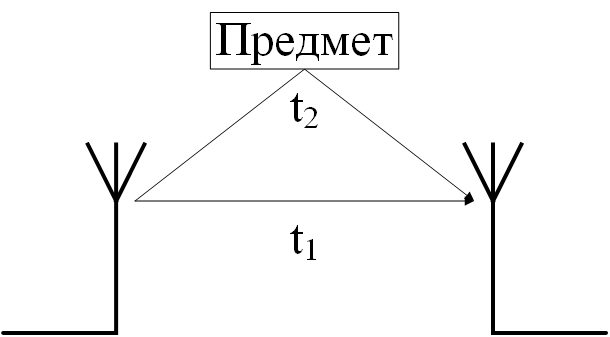
\includegraphics[width=0.6\linewidth]{AfanasyevMM/img/structure_scheme}
	\caption{Многолучевая передача}
	\label{fig:AfanasyevMM.structure_scheme}
\end{figure}

\textbf{Решение:}
Рассмотрим рисунок \ref{fig:AfanasyevMM.time_scheme}.
На нем изображен исходный передаваемый сигнал $S(t)$ с периодом $T$,
сигнал пришедший с задержкой $S(t-t_1)$,
отраженный сигнал пришедший с большей задержкой $S(t-t_2)$,
результирующий сигнал $S(t-t_1)+S(t-t_2)$, полученный в результате
сложения двух сигналов.
На результирующем сигнале штриховыми линиями показаны места
в которых пересекаются соответствующие периоды $S(t-t_1)$ и $S(t-t_2)$.
До тех пор пока будут существовать места пересечения соответствующих
периодов будет возможно произвести декодирование принятого сигнала.
Соответственно задержка должна быть $\tau < T$ чтобы передавать
со скоростью $V= \frac{1}{T}$ бит/с.
По условию задания, до появления отражения сигнала от предмета
скорость передачи была $V=1$ бит/с, откуда можно получить, что
$T= \frac{1}{8}$ с.
В результате задержки $\tau$, скорость передачи
снизилась до $V=1$ бит/с, откуда можно получить, что $T=1$ с.
Введем допущение о том, что период сигнала $T$ кратен $\frac{1}{8}$ с,
тогда получим, что $\frac{7}{8} \leq \tau < 1$.
Предположим, что $\tau > 1$ c., тогда $V<1$ бит/с, что не подходит
по условию задания.
Предположим, что $\tau < \frac{7}{8}$ с., тогда $V>1$ бит/с, что
не подходит по условию задания.

\begin{figure}[hp]
	\centering
	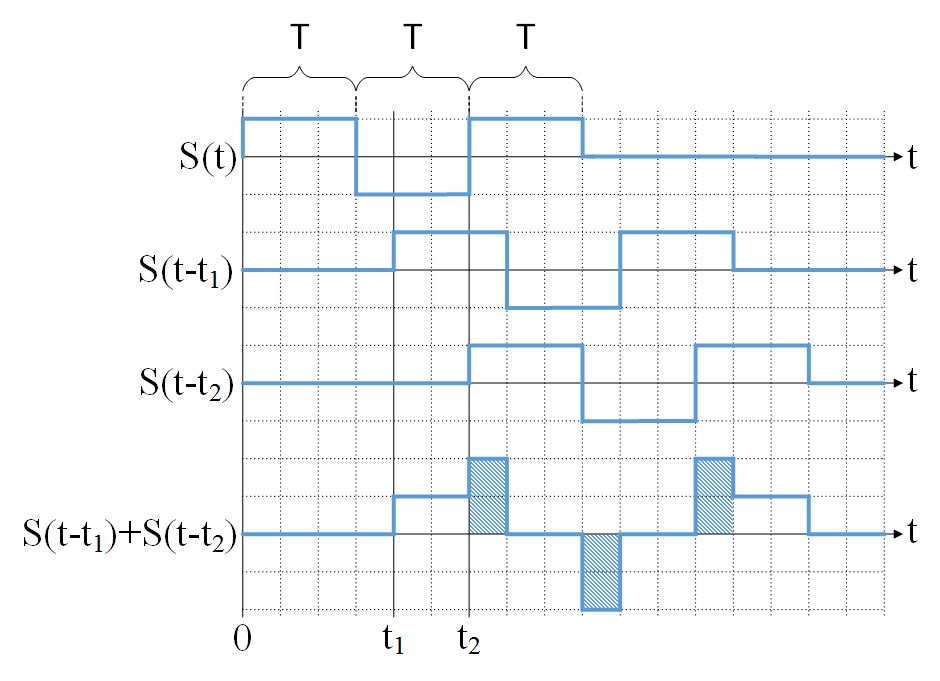
\includegraphics[width=1\linewidth]{AfanasyevMM/img/time_scheme}
	\caption{Многолучевая передача}
	\label{fig:AfanasyevMM.time_scheme}
\end{figure}